\documentclass[dvipdfmx]{jsarticle}
\usepackage[dvipdfmx]{graphicx}
\usepackage{amsmath,amssymb,amsfonts,amsthm,enumerate}
\usepackage{float}
\usepackage{bm}
\usepackage{multirow}
\usepackage{hhline}
\usepackage{diagbox}
\usepackage{caption}
\usepackage{algorithm}
\usepackage{algpseudocode}
\usepackage{colortbl}
\usepackage[subrefformat=parens]{subcaption}
\captionsetup{compatibility=false}

\setlength\floatsep{0pt} %dblfloatsep

\newcommand{\argmax}{\mathop{\rm arg~max}\limits}
\newcommand{\argmin}{\mathop{\rm arg~min}\limits}

\newenvironment{hangall}[1]{\hangindent = #1zw\everypar{\hangindent = #1zw}}{}

\setlength{\topmargin}{-25mm}
\setlength{\textheight}{270mm}
\setlength{\oddsidemargin}{-10mm}
\setlength{\textwidth}{170mm}

\bibliographystyle{jplain}
\begin{document}

\begin{center}
  \begin {tabular}[h]{|c|c|c|c|c|c|c|c|}
  \multicolumn{8}{l}{}\\
  \hline
  \multicolumn{7}{|c|}{\begin{minipage}{120mm}\vspace{.2zh}TITLE\\[-3.1zh]\begin{center}
        %%%%%%%%%%%%%%%%%%%%%%%%%%%%%%%%%%%%%%%%%%
        先行研究と今後の計画
        %%%%%%%%%%%%%%%%%%%%%%%%%%%%%%%%%%%%%%%%%%
      \end{center}\end{minipage}}
  &\begin{minipage}{20mm}Rep-No.\\[-.5zh]\hspace{3.5em}
    %%%%%%%%%%%%%%%%%%%%%
    1
    %%%%%%%%%%%%%%%%%%%
  \end{minipage}\\\hline
  \multicolumn{8}{|c|}{\begin{minipage}{120mm}\vspace{.2zh}AFFILIATION\\[-3.1zh]\begin{center}
        %%%%%%%%%%%%%%%%%%%%%%%%%%%%%%%%%%%%%%%%%%
        九州大学大学院 システム情報科学府 鈴木研究室
        %%%%%%%%%%%%%%%%%%%%%%%%%%%%%%%%%%%%%%%%%%
      \end{center}\end{minipage}}
  \\\hline
  \multicolumn{3}{|c}{\begin{minipage}{60mm}\vspace{.2zh}AUTHOR\\[-.7zh]
      \hspace{7em}Ichinsoe Haruki\end{minipage}}
  &\multicolumn{2}{|r}{\begin{minipage}{40mm}POSITION\\[-.7zh]\hspace{7.5em}B4\end{minipage}}
  &\multicolumn{3}{|c|}{\begin{minipage}{60mm}DATE\\[-.7zh]\hspace{9em}
      %%%%%%%%%%%%%%%%%%%%%%%%%%%%%%%%%%%%%
      2025/05/14
      %%%%%%%%%%%%%%%%%%%%%%%%%%%%%%%%%%%%%

    \end{minipage}}\\\hline
  \end{tabular}
\end{center}

\section{先行研究:データの偏見的説明の判定}

本節では, Roslingらの『Factfulness』で提唱された10の人間の本能(ギャップ本能、恐怖本能、単一視点本能など)\cite{rosling2018}が悪用されることで, 統計的に非倫理的であり偏りがあるが, 一定数の人が信じてしまうような偏見的説明になっているか否かということを判定するZhangらの2つの研究を先行研究として紹介する\cite{zhang2022, zhang2023}.

\subsection{フレーズ間の意味的類似度に基づくデータの偏見的説明判定}
Zhangら(2022)は, このような非倫理的であり偏りがあるが, 一定数の人が信じてしまう偏見的説明を18個(Type I~XVIII)定義し, さらに, その説明が偏見的説明か否かを判定する3つの手法($\alpha$),($\beta$),($\gamma$)を提案している\cite{zhang2022}.
\begin{enumerate}
  \renewcommand{\labelenumi}{(\arabic{enumi})}
  \item 手法($\alpha$)

        法$\alpha$は, 習慣Xと病気Yに関する解説文を判定する手法であり, 以下の3つの指標によって判定する。
        \vspace{1em}
        \begin{itemize}
          \item 習慣と病気の関連度:$\theta_{\text{relevance}}$
          \item 恐怖度:$\theta_{\text{bad~habit}}$
          \item 悪い習慣度:$\theta_{\text{fear}}$

        \end{itemize}
        \vspace{1em}

        それぞれの指標は次のように定義される.
        \begin{equation*}
          \theta_{\text{relevance}} = \frac{\text{Sim}(X, Y)}{\text{Sim}(\text{base word},Y)}
        \end{equation*}

        \begin{equation*}
          \theta_{\text{bad~habit}} = \frac{\text{Sim}(X, \text{``bad habit''})}{\text{Sim}(X, \text{``good habit''})}
        \end{equation*}

        \begin{equation*}
          \theta_{\text{fear}} \Rightarrow \text{DALYs(障害調整生存年数)に基づくスコア}
        \end{equation*}

        これら3つの値がそれぞれ1を超えた場合, その説明は偏見的説明であると判定される. この条件を, 以下のように表す.

        \begin{align*}
           & \text{IF} \quad \theta_{\text{relevance}} > 1 \quad \land \quad \theta_{\text{bad~habit}} > 1 \quad \land \quad \theta_{\text{fear}} > 1 \\
           & \text{THEN} \quad 1                                                                                                                      \\
           & \text{ELSE} \quad 0
        \end{align*}

  \item 手法($\beta$)

        手法$\beta$は、「主語 $X$ が他のいくつかの主語 $X'$ と比較して性質 $Y$ を持つ」ことを説明する解説文を判定する手法であり, 次の2つの条件がともに成立する場合にのみ, その説明を偏見的説明と判定する.
        \vspace{1em}
        \begin{itemize}
          \item[(1)] 主語 $X$ が, 逆の性質 $\bar{Y}$ よりも性質 $Y$ に関連していること.
          \item[(2)] 性質 $Y$ が, 他クラスに属するすべての主語 $X'$ よりも主語 $X$ に強く関連していること.
        \end{itemize}
        \vspace{1em}

        これを $X$と$Y$の関連度$\theta^{\beta}_{XY}$, $X$と$\bar{Y}$の関連度$\theta^{\beta}_{X\bar{Y}}$, $X'$と$Y$の関連度$\theta^{\beta}_{X'Y}$を用いて以下のように表す.

        \begin{align}
           & \text{IF} \quad \theta_{XY} > \theta_{X\bar{Y}} \quad \land \quad \forall X' \left( \theta_{XY} > \theta_{X'Y} \right) \\
           & \text{THEN} \quad 1                                                                                                    \\
           & \text{ELSE} \quad 0 \tag{2.2}
        \end{align}

        \vspace{1em}

  \item 手法($\gamma$)

        手法$\gamma$は, 「主語$X$が他の種類の傾向$Y'$とは異なる傾向$Y$をもつ」ことを説明する解説文を判定する手法であり, 主語$X$が, 異なるどの傾向$Y'$よりも傾向$Y$と強く関連する場合のみ, 偏見的説明と判定する. この条件を, $X$と$Y$の関連度$\theta^{\gamma}_{XY}$, $X$と$Y$の関連度$\theta^{\gamma}_{XY'}$を用いて以下で表す.

        \begin{align}
           & \text{IF} \quad \forall Y' \left( \theta_{XY} > \theta_{XY'} \right) \\
           & \text{THEN} \quad 1                                                  \\
           & \text{ELSE} \quad 0
        \end{align}

\end{enumerate}

これらの手法を用いて, 定義した解説文とそのフレーズを一部変えた変種に対して実験を行った結果, ($\alpha$)と($\gamma$)は正答率1, 0.914と比較的高い結果を残したが, ($\beta$)は, 正答率0.510という結果となった. これは,($\beta$)が限られてフレーズ間の意味的類似性のみ測定を行っているためであると考えられた.

\subsection{類義語フレーズ類似度に基づくデータの偏見的説明判定}
その後の研究でZhangらは、特に手法($\beta$)における判定精度の低さを改善するため、Phrase Similarity Graphを導入し, 新たな判定手法(${\beta}^2$)を提案した\cite{zhang2023}.
\vspace{1em}

これは, 主語, 比較主語, 目的語, 性質, 比較性質を表す$X$, $X'$, ${Y}_{\text{base}}$, $Y$, $\bar{Y}$のそれぞれに対して, ChatGPTを基に類義語を含んだフレーズ群を生成し, 幅広いフレーズ間で意味的関係を探索するものである. 生成の過程では, 元々の語と類似語群の間に3層のフレーズ類似度グラフを作成し, それを図1のような部分グラフに分解を行った. その後, グラフエントロピーを求めて, 偏りのある部分グラフに重み付けを行い, 信頼生成スコアを測定した.

\begin{figure}[H]
  \centering
  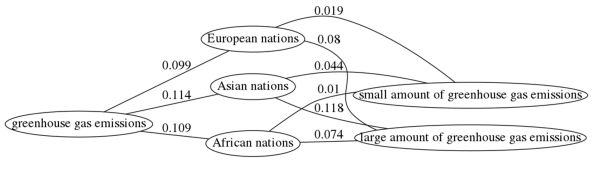
\includegraphics[width=0.8\linewidth]{01.png}
  \caption{サブグラフの例}
  \label{fig:subgraph}
\end{figure}

この改良により、従来の$\beta$手法の精度が81.1\%まで向上し, 直感に反する類似度の問題を緩和できることが示された.

\section{先行研究:データの偏見的説明に関する系統的分類とLLM生成}

樋口氏の修士論文では, Zhangらの分類を基に図2に示すようにデータの偏見的説明を対象$S$(1つか2つ以上), 時間的拡張の有無$T$(ありかなし)に基づき4つのパターンに系統的に分類する手法を提案している\cite{higuchi2024}.

\begin{figure}[H]
  \centering
  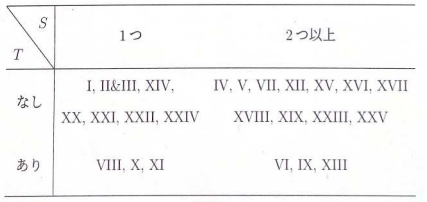
\includegraphics[width=0.6\linewidth]{02.png}
  \caption{データの偏見的説明の分類}
  \label{fig:pattern2}
\end{figure}

また, この系統的分類を基に図3に示すような本能決定の手続きを定め, LLMを用いてデータの偏見的説明の生成を行った.

\begin{figure}[H]
  \centering
  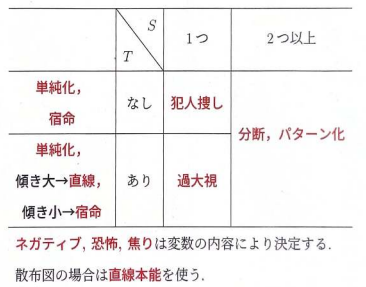
\includegraphics[width=0.6\linewidth]{03.png}
  \caption{本能の決定手続き}
  \label{fig:instinct-flow}
\end{figure}


LLMを用いて生成を行う過程では, ペルソナ設計とChain-of-Thoughtによるプロンプトエンジニアリングを実施して出力精度の向上を図っている.
\vspace{1em}
その結果, 提案した分類パターンと本能決定手続きをプロンプト構造に明示的に組み込むことで, 意図した偏見的説明パターンに沿った説明文が高い一貫性で生成されることが確認された. 以下に結果の一例として, "gpt-4o-mini"を用いた際の結果を判定方法毎に示す.

\begin{figure}[H]
  \centering
  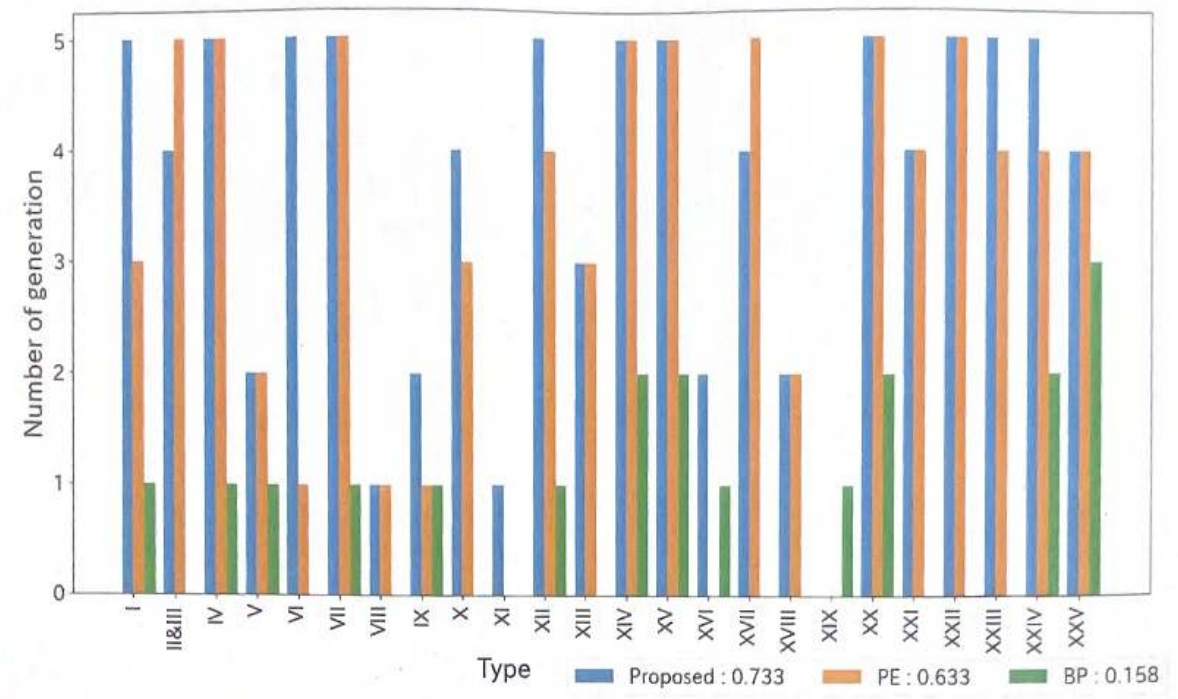
\includegraphics[width=0.6\linewidth]{04.png}
  \caption{LLM:gpt-4o-mini, 判定方法:自身}
  \label{fig:pattern4}
\end{figure}

\begin{figure}[H]
  \centering
  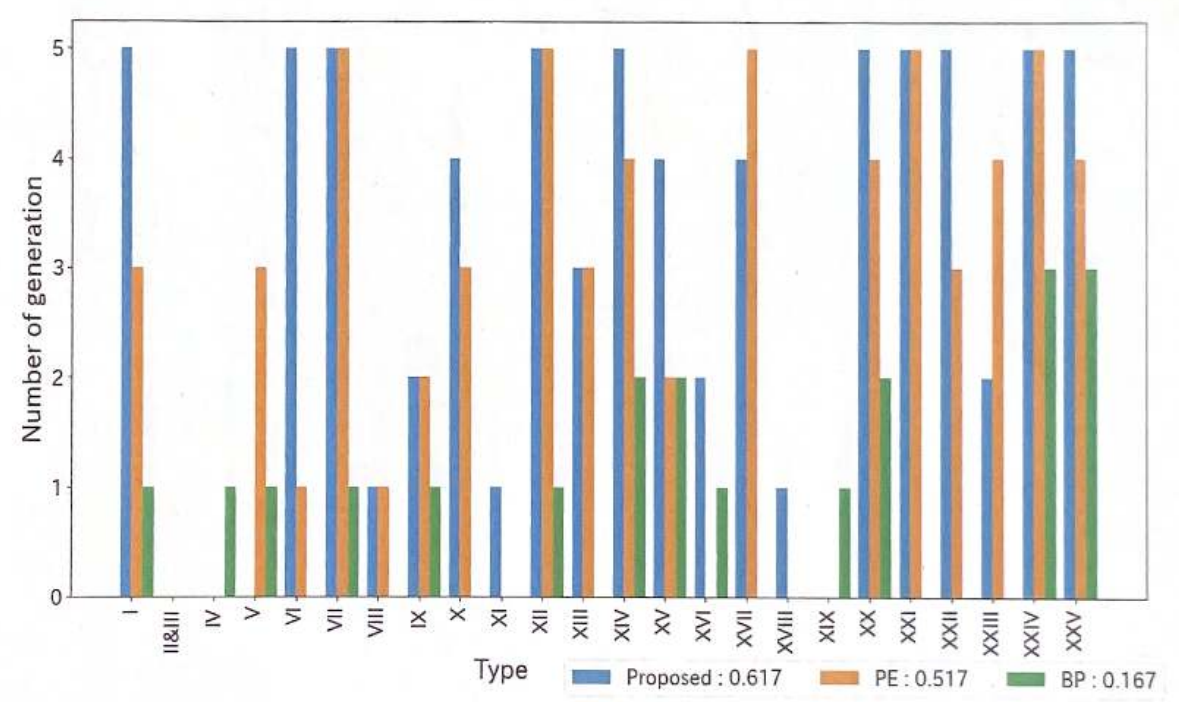
\includegraphics[width=0.6\linewidth]{05.png}
  \caption{LLM:gpt-4o-mini, 判定方法:LLM}
  \label{fig:pattern5}
\end{figure}

以上より, 本研究で提案された分類フレームワークとプロンプト設計手法は, 偏見的説明の多様なパターンを体系的に再現・制御可能であることを実証し, 今後の説明文生成タスクや偏見評価タスクにおいて有用な基盤となりうると結論づけられる.






\section{今後の計画:一般時事ニュースからの偏見的説明の生成}

これまでの先行研究を踏まえて, 私は統計データに基づく一般時事ニュースの中から, 信憑性が高く見える一方で, 読者に偏った印象を与えるような説明を生成することを今後のテーマに据えようと考えている.
\vspace{1em}
実現を目指す流れは以下の3段階から成る.

\begin{enumerate}
  \item \textbf{統計データからの要素抽出と本能決定}:
        時事データから, 主語・性質・対象群などの要素を構造的に抽出し, それに対応する人間の本能を決定する。

  \item \textbf{偏見的説明文の生成}:
        抽出された要素と選定された本能に基づき, データの一部のみを強調・誇張するような説明文を生成する.

  \item \textbf{生成された説明の判定}:
        Zhangらの手法($\alpha$, $\beta$, $\gamma$, ${\beta}^2$)やLLMを用いて, 生成された説明文が偏見的説明であるかを判定する.
\end{enumerate}

この一連のフローにより, 単なる誤情報や虚偽ではないが, 受け手の直感や判断を不適切に誘導する説明文を系統的に生成・分析・判定する枠組みの実現を目指している.

\vspace{1em}
今後の課題としては,以下の点が挙げられる.

\begin{itemize}
  \item 統計データからどのように有効な構成要素(主語・性質・比較対象など)を抽出し, それに対して適切な本能ラベルを自動的に割り当てるか
  \item 抽出要素と本能に基づいて, どのようなモデル(LLM, VLM, Deep Learning等)を用いれば, 効果的かつ制御可能に偏見的説明文を生成できるか
  \item 具体的にどのような一般時事ニュースのデータを利用していくか(米の価格推移、外国人労働者数と犯罪件数の変化など)
\end{itemize}

なお, 本研究における偏見的説明文の生成は, あくまで「そのような説明がどのように構成され, どのような要素が人間の認知に影響を与えるか」を明らかにし, ひいてはそのような説明文の生成の防止や検知につながることを期待しており, 不適切な説明文の自動生成自体を目的とするものではない.

\begin{thebibliography}{99}
  \bibitem{rosling2018}
  H. Rosling, A. R. Rönnlund, and O. Rosling. \textit{Factfulness: Ten Reasons We’re Wrong About the World—and Why Things Are Better Than You Think}. Sceptre, London, United Kingdom, 2018.

  \bibitem{zhang2022}
  K. Zhang, H. Shinden, T. Mutsuro, and E. Suzuki. Judging Instinct Exploitation in Statistical Data Explanations Based on Word Embedding. In \textit{Proc. AIES ’22}, pp. 867–879, 2022.

  \bibitem{zhang2023}
  K. Zhang and E. Suzuki. Judging Credible and Unethical Statistical Data Explanations via Phrase Similarity Graph. In \textit{Proc. 2023 Pacific Asia Conference on Information Systems (PACIS)}, 2023.

  \bibitem{higuchi2024}
  T. Higuchi. \textit{データの偏見的説明に関する系統的分類とLLM生成}.
  Master's Thesis, Kyushu University, Graduate School of Information Science and Electrical Engineering, 2024.


\end{thebibliography}
\end{document}